\documentclass[aspectratio=169, 10pt]{beamer}

% ---------- Theme ----------
\usetheme{metropolis}
\usepackage{tikz}
\usetikzlibrary{arrows.meta, positioning, fit, backgrounds, shapes.multipart, calc}
\usepackage{booktabs}

\definecolor{crwblue}{HTML}{2563EB}
\definecolor{crwdark}{HTML}{1E293B}
\definecolor{crwgreen}{HTML}{16A34A}
\definecolor{crwamber}{HTML}{D97706}
\definecolor{crwred}{HTML}{DC2626}
\definecolor{crwpurple}{HTML}{7C3AED}
\definecolor{crwgray}{HTML}{64748B}
\definecolor{crwbg}{HTML}{F8FAFC}

\setbeamercolor{palette primary}{bg=crwdark, fg=white}
\setbeamercolor{frametitle}{bg=crwdark, fg=white}
\setbeamercolor{progress bar}{fg=crwblue, bg=crwgray!30}
\setbeamercolor{alerted text}{fg=crwblue}
\setbeamertemplate{frame numbering}[fraction]

\title{Centralized Research Workspace}
\subtitle{An Architectural Deep Dive into a Layered, Secure, Multi-Tenant Research Platform}
\author{Team noWayHome \;\textbar\; Rafat Abdullah \(\cdot\) Mahiul Kabir \(\cdot\) Sohom Sattyam}
\date{CSE 4636 --- Web Architecture}

% ---------- TikZ styles ----------
\tikzset{
  layer/.style={rectangle, rounded corners=3pt, minimum width=8.6cm, minimum height=1.05cm,
    draw=crwdark, line width=0.8pt, font=\bfseries\small, align=center, text=white},
  sublayer/.style={rectangle, rounded corners=2pt, minimum width=3.6cm, minimum height=0.9cm,
    draw=crwdark!60, line width=0.6pt, font=\small, align=center},
  ent/.style={rectangle, rounded corners=2pt, draw=crwdark, line width=0.7pt, minimum width=2.5cm,
    minimum height=0.85cm, font=\scriptsize\bfseries, align=center, fill=white},
  hub/.style={rectangle, rounded corners=3pt, draw=crwblue, line width=1.1pt, minimum width=3cm,
    minimum height=1cm, font=\bfseries\small, align=center, fill=crwblue!10},
  arr/.style={-{Latex[length=2mm]}, line width=0.7pt, crwgray},
  bigarr/.style={-{Latex[length=2.5mm]}, line width=1pt, crwdark},
}

\begin{document}

% ============================================================
\begin{frame}
  \titlepage
\end{frame}

% ============================================================
\begin{frame}{What Is CRW?}
  \begin{columns}[T,onlytextwidth]
    \column{0.56\textwidth}
      \textbf{The problem:} academic researchers juggle separate tools for literature review, task tracking, manuscript drafting, and meeting notes --- constant \alert{app-switching fatigue}.

      \vspace{0.4cm}
      \textbf{The solution:} one collaborative workspace, four integrated modules, one consistent access-control model.

      \vspace{0.4cm}
      \begin{itemize}\setlength\itemsep{4pt}
        \item[$\bullet$] Kanban / list task tracking
        \item[$\bullet$] Literature repository with threaded annotations
        \item[$\bullet$] Versioned manuscript drafting (Markdown)
        \item[$\bullet$] Meeting minutes \& decisions log
        \item[$\bullet$] Cross-module global search
      \end{itemize}
    \column{0.4\textwidth}
      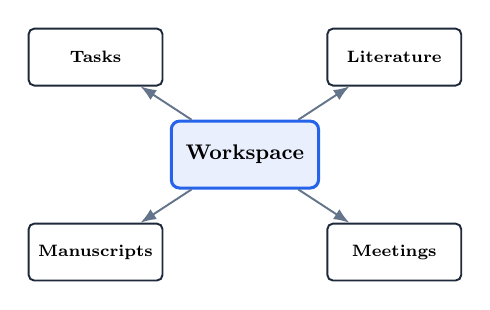
\begin{tikzpicture}[scale=0.85, every node/.style={transform shape}]
        \node[hub, minimum width=2.2cm] (ws) {Workspace};
        \node[ent, minimum width=2cm, above left=0.5cm and 0.1cm of ws] (t) {Tasks};
        \node[ent, minimum width=2cm, above right=0.5cm and 0.1cm of ws] (l) {Literature};
        \node[ent, minimum width=2cm, below left=0.5cm and 0.1cm of ws] (m) {Manuscripts};
        \node[ent, minimum width=2cm, below right=0.5cm and 0.1cm of ws] (mt) {Meetings};
        \draw[arr] (ws) -- (t);
        \draw[arr] (ws) -- (l);
        \draw[arr] (ws) -- (m);
        \draw[arr] (ws) -- (mt);
      \end{tikzpicture}
      \small\centering \textit{The Workspace is the tenancy boundary every module hangs off of.}
  \end{columns}
\end{frame}

% ============================================================
\begin{frame}{Why This Deck Is About Architecture}
  This talk deliberately skips feature tours and focuses on \alert{how the system is built}:
  \begin{enumerate}\setlength\itemsep{8pt}
    \item A strict \textbf{layered backend} (Controller $\to$ Service $\to$ Repository $\to$ Entity)
    \item An \textbf{API-contract layer of DTOs} that never leaks persistence models
    \item \textbf{Stateless JWT security} composed with \textbf{method-level authorization}
    \item A hand-rolled \textbf{multi-tenancy guard} enforcing workspace-scoped access
    \item Centralized \textbf{exception handling} for a uniform error contract
    \item A \textbf{React context + interceptor} architecture on the frontend
    \item A single \textbf{cross-cutting search} that respects all of the above
  \end{enumerate}
\end{frame}

% ============================================================
\begin{frame}{Technology Stack}
  \begin{columns}[T,onlytextwidth]
    \column{0.5\textwidth}
      \textbf{Backend}
      \begin{itemize}\setlength\itemsep{4pt}
        \item Java 17, Spring Boot 3.3
        \item Spring Data JPA (Hibernate)
        \item Spring Security 6 (JWT, \texttt{@EnableMethodSecurity})
        \item H2 --- \textbf{file-backed}, not in-memory
        \item JJWT 0.12, Lombok, Bean Validation
      \end{itemize}
    \column{0.5\textwidth}
      \textbf{Frontend}
      \begin{itemize}\setlength\itemsep{4pt}
        \item React 18 + Vite
        \item React Router (protected routes)
        \item Axios with request interceptors
        \item React Context for global state
        \item React Markdown for rendering
      \end{itemize}
  \end{columns}
  \vspace{0.5cm}
  \begin{center}
  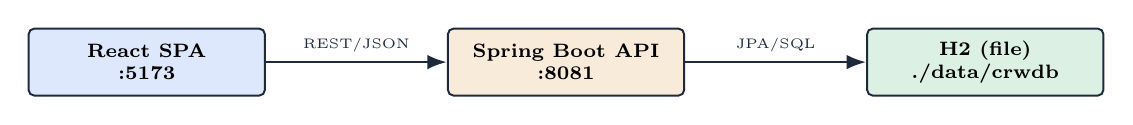
\begin{tikzpicture}
    \node[ent, fill=crwblue!15, minimum width=3cm] (fe) {React SPA \\ \scriptsize:5173};
    \node[ent, fill=crwamber!15, minimum width=3cm, right=2.3cm of fe] (be) {Spring Boot API \\ \scriptsize:8081};
    \node[ent, fill=crwgreen!15, minimum width=3cm, right=2.3cm of be] (db) {H2 (file) \\ \scriptsize ./data/crwdb};
    \draw[bigarr] (fe) -- node[above,font=\tiny]{REST/JSON} (be);
    \draw[bigarr] (be) -- node[above,font=\tiny]{JPA/SQL} (db);
  \end{tikzpicture}
  \end{center}
\end{frame}

% ============================================================
\begin{frame}{System Architecture --- 30,000 ft View}
  \centering
  \resizebox{!}{0.76\textheight}{%
  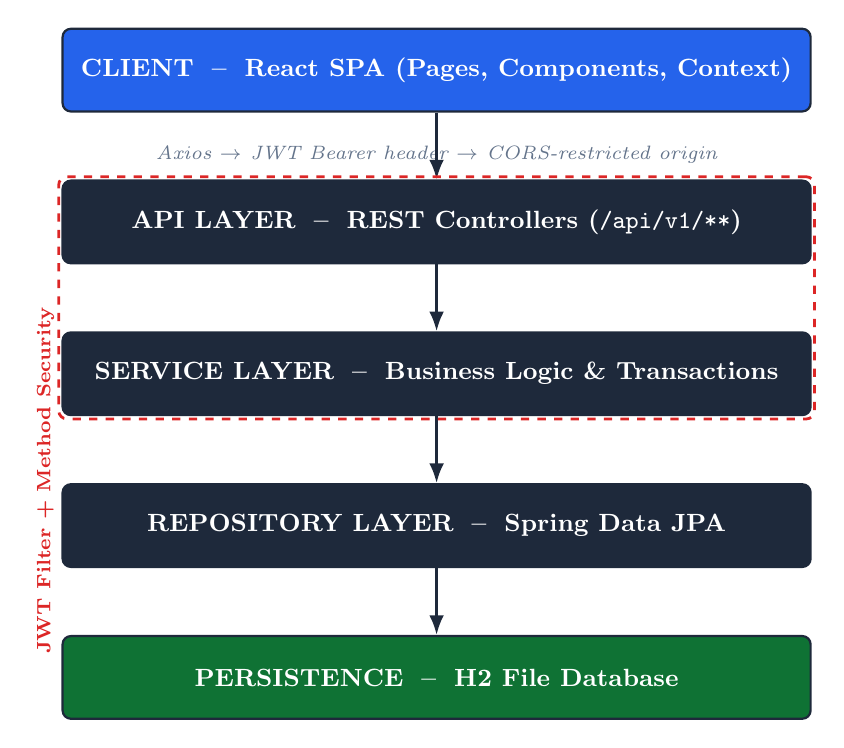
\begin{tikzpicture}
    % Client
    \node[layer, fill=crwblue, minimum width=9.5cm] (client) {CLIENT \;--\; React SPA (Pages, Components, Context)};
    % Network
    \node[below=0.3cm of client, font=\scriptsize\itshape, crwgray] (net) {Axios $\to$ JWT Bearer header $\to$ CORS-restricted origin};
    % API layer
    \node[layer, fill=crwdark, below=0.85cm of client, minimum width=9.5cm] (api) {API LAYER \;--\; REST Controllers (\texttt{/api/v1/**})};
    % Service layer
    \node[layer, fill=crwdark, below=0.85cm of api, minimum width=9.5cm] (svc) {SERVICE LAYER \;--\; Business Logic \& Transactions};
    % Repository layer
    \node[layer, fill=crwdark, below=0.85cm of svc, minimum width=9.5cm] (repo) {REPOSITORY LAYER \;--\; Spring Data JPA};
    % DB
    \node[layer, fill=crwgreen!70!black, below=0.85cm of repo, minimum width=9.5cm] (db) {PERSISTENCE \;--\; H2 File Database};

    \draw[bigarr] (client) -- (api);
    \draw[bigarr] (api) -- (svc);
    \draw[bigarr] (svc) -- (repo);
    \draw[bigarr] (repo) -- (db);

    % Security filter overlay
    \node[fit=(api)(svc), draw=crwred, dashed, rounded corners=3pt, line width=1pt, inner sep=1pt] (secbox) {};
    \node[crwred, font=\scriptsize\bfseries, left=0.15cm of secbox, rotate=90] {JWT Filter + Method Security};
  \end{tikzpicture}%
  }

  \vspace{0.4cm}
  \small Every horizontal boundary is a \alert{contract}: DTOs cross the API boundary, entities never do.
\end{frame}

% ============================================================
\begin{frame}{Backend: Strict Layered Design}
  \begin{columns}[T,onlytextwidth]
    \column{0.62\textwidth}
      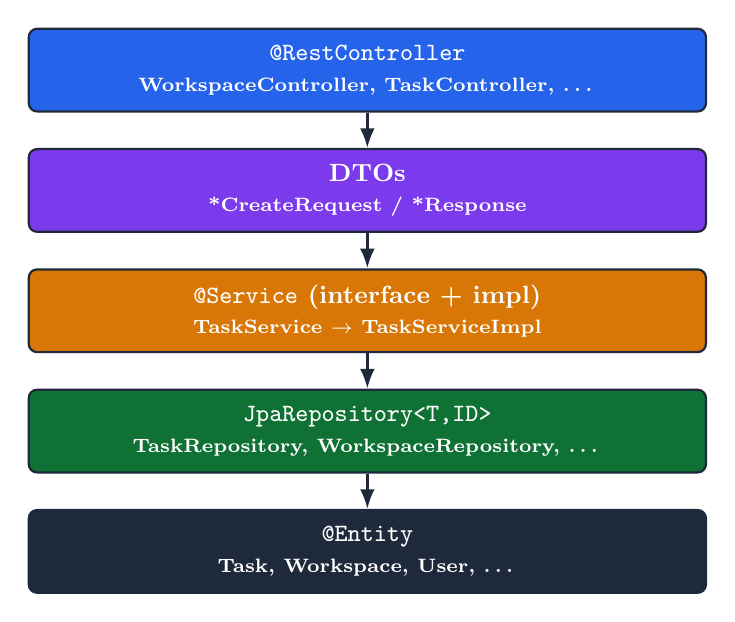
\begin{tikzpicture}[node distance=0.45cm]
        \node[layer, fill=crwblue] (ctrl) {\texttt{@RestController}\\ \scriptsize WorkspaceController, TaskController, \dots};
        \node[layer, fill=crwpurple, below=of ctrl] (dto) {DTOs \\ \scriptsize *CreateRequest / *Response};
        \node[layer, fill=crwamber, below=of dto] (svc) {\texttt{@Service} (interface + impl) \\ \scriptsize TaskService $\to$ TaskServiceImpl};
        \node[layer, fill=crwgreen!70!black, below=of svc] (repo) {\texttt{JpaRepository<T,ID>} \\ \scriptsize TaskRepository, WorkspaceRepository, \dots};
        \node[layer, fill=crwdark, below=of repo] (ent) {\texttt{@Entity} \\ \scriptsize Task, Workspace, User, \dots};
        \foreach \a/\b in {ctrl/dto, dto/svc, svc/repo, repo/ent}
          \draw[bigarr] (\a) -- (\b);
      \end{tikzpicture}
    \column{0.38\textwidth}
      \small
      \textbf{Why it matters:}
      \begin{itemize}\setlength\itemsep{6pt}
        \item Every domain (\emph{Task, Literature, Manuscript, Meeting, Workspace, User, Chat}) repeats the \alert{same 5-layer skeleton}
        \item Controllers stay thin: validate input, delegate, map to DTO
        \item Services own transactions \& business rules (e.g.\ reassigning a task, publishing a manuscript version)
        \item Interfaces (\texttt{TaskService}) decouple contracts from implementation --- testable, swappable
      \end{itemize}
  \end{columns}
\end{frame}

% ============================================================
\begin{frame}{Why DTOs? Isolating the API Contract}
  \begin{columns}[T,onlytextwidth]
    \column{0.48\textwidth}
      \textbf{Without DTOs} \textcolor{crwred}{$\times$}
      \begin{itemize}\setlength\itemsep{5pt}
        \item Entities serialized directly to JSON
        \item Lazy-loaded collections trigger \texttt{LazyInitializationException} or N+1 explosions
        \item Password hashes, internal IDs, JPA proxies leak to clients
        \item Any schema change breaks the frontend
      \end{itemize}
    \column{0.48\textwidth}
      \textbf{With DTOs} \textcolor{crwgreen}{$\checkmark$}
      \begin{itemize}\setlength\itemsep{5pt}
        \item \texttt{*CreateRequest} validates inbound payloads (\texttt{@NotBlank}, \texttt{@Valid})
        \item \texttt{*Response} shapes exactly what the UI needs
        \item Entity graph can evolve independently of the wire format
        \item Sensitive fields (e.g.\ \texttt{User.password}) are structurally unreachable
      \end{itemize}
  \end{columns}
  \vspace{0.4cm}
  \begin{center}
  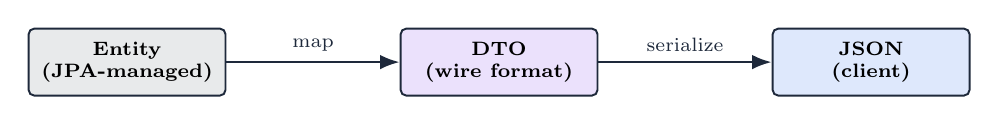
\begin{tikzpicture}
    \node[ent, fill=crwdark!10] (ent) {Entity \\ \scriptsize (JPA-managed)};
    \node[ent, fill=crwpurple!15, right=2.2cm of ent] (dto) {DTO \\ \scriptsize (wire format)};
    \node[ent, fill=crwblue!15, right=2.2cm of dto] (json) {JSON \\ \scriptsize (client)};
    \draw[bigarr] (ent) -- node[above, font=\scriptsize]{map} (dto);
    \draw[bigarr] (dto) -- node[above, font=\scriptsize]{serialize} (json);
  \end{tikzpicture}
  \end{center}
\end{frame}

% ============================================================
\begin{frame}{Domain Model: Workspace as the Tenancy Root}
  \centering
  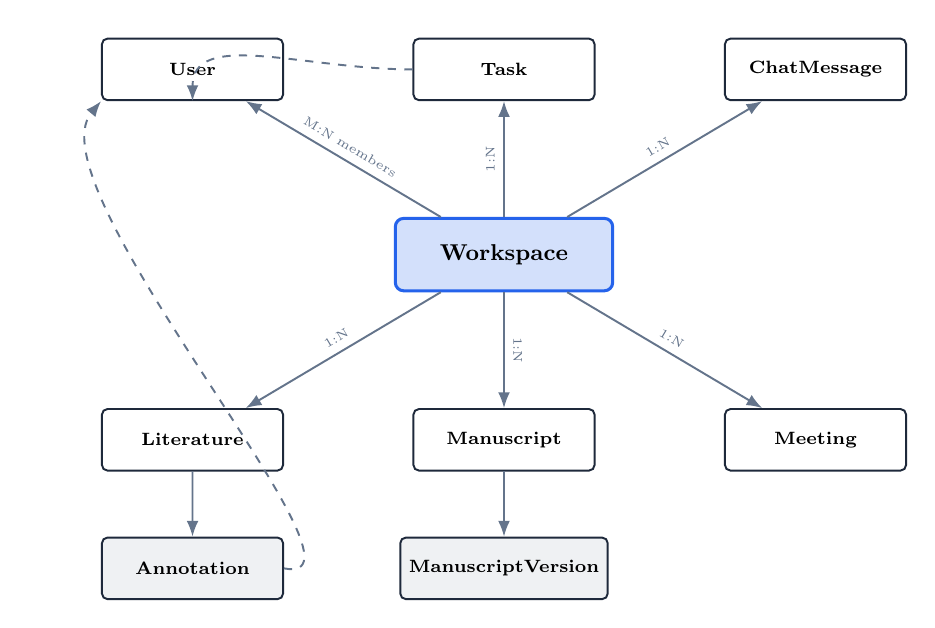
\begin{tikzpicture}[node distance=1.3cm, scale=0.92, every node/.style={transform shape}]
    \node[hub, fill=crwblue!20] (ws) {Workspace};
    \node[ent, above=1.6cm of ws, xshift=-4.3cm] (user) {User};
    \node[ent, above=1.6cm of ws, xshift=0cm] (task) {Task};
    \node[ent, above=1.6cm of ws, xshift=4.3cm] (chat) {ChatMessage};
    \node[ent, below=1.6cm of ws, xshift=-4.3cm] (lit) {Literature};
    \node[ent, below=1.6cm of ws, xshift=0cm] (man) {Manuscript};
    \node[ent, below=1.6cm of ws, xshift=4.3cm] (meet) {Meeting};
    \node[ent, below=0.9cm of lit, fill=crwgray!10] (ann) {Annotation};
    \node[ent, below=0.9cm of man, fill=crwgray!10] (ver) {ManuscriptVersion};

    \draw[arr] (ws) -- node[font=\tiny, above, sloped]{M:N members} (user);
    \draw[arr] (ws) -- node[font=\tiny, above, sloped]{1:N} (task);
    \draw[arr] (ws) -- node[font=\tiny, above, sloped]{1:N} (chat);
    \draw[arr] (ws) -- node[font=\tiny, above, sloped]{1:N} (lit);
    \draw[arr] (ws) -- node[font=\tiny, above, sloped]{1:N} (man);
    \draw[arr] (ws) -- node[font=\tiny, above, sloped]{1:N} (meet);
    \draw[arr] (lit) -- (ann);
    \draw[arr] (man) -- (ver);
    \draw[arr, dashed] (task.west) .. controls +(-1.5,0) and +(0,1) .. (user.south);
    \draw[arr, dashed] (ann.east) .. controls +(1.5,-0.3) and +(-1,-1.2) .. (user.south west);
  \end{tikzpicture}

  \small Solid = ownership (\texttt{@OneToMany}/\texttt{@ManyToMany}) \quad Dashed = attribution (\texttt{assignee}/\texttt{author})
\end{frame}

% ============================================================
\begin{frame}{Security Architecture: Stateless JWT Flow}
  \centering
  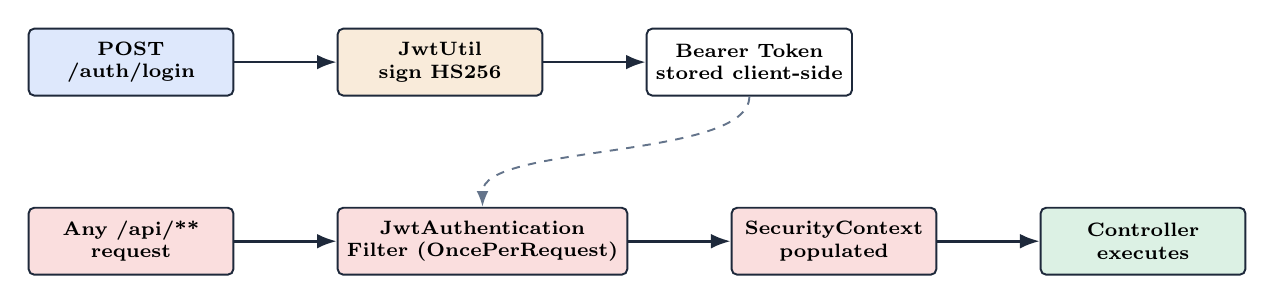
\begin{tikzpicture}[node distance=0.9cm, font=\small]
    \node[ent, fill=crwblue!15, minimum width=2.6cm] (login) {POST \\ \scriptsize /auth/login};
    \node[ent, fill=crwamber!15, right=1.3cm of login, minimum width=2.6cm] (jwtutil) {JwtUtil \\ \scriptsize sign HS256};
    \node[ent, fill=white, right=1.3cm of jwtutil, minimum width=2.6cm] (token) {Bearer Token \\ \scriptsize stored client-side};
    \draw[bigarr] (login) -- (jwtutil);
    \draw[bigarr] (jwtutil) -- (token);

    \node[ent, fill=crwred!15, below=1.4cm of login, minimum width=2.6cm] (req) {Any /api/** \\ \scriptsize request};
    \node[ent, fill=crwred!15, right=1.3cm of req, minimum width=2.6cm] (filter) {JwtAuthentication\\Filter \scriptsize (OncePerRequest)};
    \node[ent, fill=crwred!15, right=1.3cm of filter, minimum width=2.6cm] (ctx) {SecurityContext \\ \scriptsize populated};
    \node[ent, fill=crwgreen!15, right=1.3cm of ctx, minimum width=2.6cm] (ctrl) {Controller \\ \scriptsize executes};
    \draw[bigarr] (req) -- (filter);
    \draw[bigarr] (filter) -- (ctx);
    \draw[bigarr] (ctx) -- (ctrl);

    \draw[arr, dashed] (token.south) .. controls +(0,-0.8) and +(0,0.8) .. (filter.north);
  \end{tikzpicture}
  \vspace{0.4cm}
  \begin{itemize}\setlength\itemsep{4pt}
    \item \texttt{SessionCreationPolicy.STATELESS} --- no server-side session, horizontally scalable by design
    \item Filter runs \textbf{before} \texttt{UsernamePasswordAuthenticationFilter}; validates signature + expiry once per request
    \item Passwords hashed with \texttt{BCryptPasswordEncoder}; CSRF disabled only for stateless \texttt{/api/**} \& \texttt{/h2-console/**}
  \end{itemize}
\end{frame}

% ============================================================
\begin{frame}{Authorization: Two Independent Guards}
  \begin{columns}[T,onlytextwidth]
    \column{0.48\textwidth}
      \textbf{1. Role-based (coarse)} \\
      \texttt{@EnableMethodSecurity} + \texttt{@PreAuthorize("hasRole('ADMIN')")}
      \begin{itemize}\setlength\itemsep{5pt}
        \item Enforced declaratively at the method boundary
        \item Distinguishes \texttt{ADMIN} vs \texttt{RESEARCHER}
        \item e.g.\ only an admin can remove a member
      \end{itemize}
    \column{0.48\textwidth}
      \textbf{2. Tenancy-based (fine)} \\
      \texttt{WorkspaceAccessGuard}
      \begin{itemize}\setlength\itemsep{5pt}
        \item Resolves the caller from \texttt{SecurityContext} $\to$ \texttt{User}
        \item \texttt{requireMember(workspace)} throws \texttt{AccessDeniedException} if the caller isn't in \texttt{workspace.members}
        \item Every service call that touches a Task/Literature/Manuscript/Meeting runs through this check first
      \end{itemize}
  \end{columns}
  \vspace{0.5cm}
  \begin{center}\small
  \alert{Role security answers ``\emph{what can this user do}''; the workspace guard answers ``\emph{what is this user's data}''.}
  \end{center}
\end{frame}

% ============================================================
\begin{frame}{Centralized Exception Handling}
  \centering
  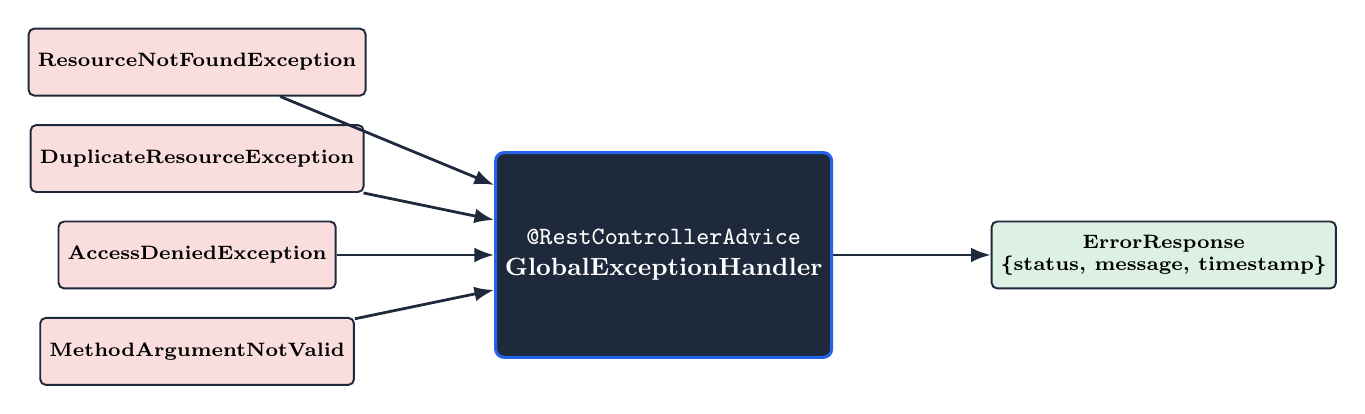
\begin{tikzpicture}[node distance=1.0cm]
    \node[ent, fill=crwred!15, minimum width=3.3cm] (rnf) {ResourceNotFoundException};
    \node[ent, fill=crwred!15, below=0.35cm of rnf, minimum width=3.3cm] (dup) {DuplicateResourceException};
    \node[ent, fill=crwred!15, below=0.35cm of dup, minimum width=3.3cm] (denied) {AccessDeniedException};
    \node[ent, fill=crwred!15, below=0.35cm of denied, minimum width=3.3cm] (val) {MethodArgumentNotValid};

    \node[hub, fill=crwdark, text=white, right=2cm of denied, minimum height=2.6cm] (geh) {\texttt{@RestControllerAdvice}\\ GlobalExceptionHandler};

    \node[ent, fill=crwgreen!15, right=2cm of geh, minimum width=3cm] (resp) {ErrorResponse \\ \scriptsize \{status, message, timestamp\}};

    \foreach \n in {rnf, dup, denied, val}
      \draw[bigarr] (\n) -- (geh);
    \draw[bigarr] (geh) -- (resp);
  \end{tikzpicture}
  \vspace{0.4cm}
  \begin{itemize}\setlength\itemsep{4pt}
    \item Every controller is exception-free of boilerplate try/catch --- one advice class maps exceptions to HTTP status codes
    \item \texttt{RestAuthenticationEntryPoint} guarantees unauthenticated calls get a clean \texttt{401 JSON} body, not a servlet-container HTML page
    \item Result: the frontend can rely on \emph{one} error shape everywhere
  \end{itemize}
\end{frame}

% ============================================================
\begin{frame}{Frontend Architecture: Context + Interceptor}
  \begin{columns}[T,onlytextwidth]
    \column{0.52\textwidth}
      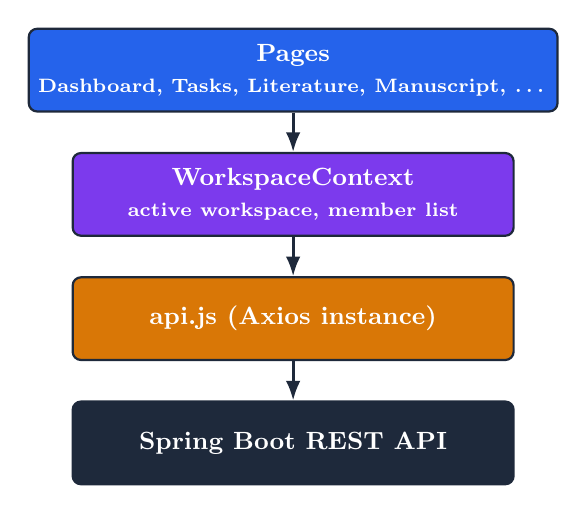
\begin{tikzpicture}[node distance=0.5cm]
        \node[layer, fill=crwblue, minimum width=5.6cm] (pages) {Pages \\ \scriptsize Dashboard, Tasks, Literature, Manuscript, \dots};
        \node[layer, fill=crwpurple, below=of pages, minimum width=5.6cm] (ctx) {WorkspaceContext \\ \scriptsize active workspace, member list};
        \node[layer, fill=crwamber, below=of ctx, minimum width=5.6cm] (svc) {api.js (Axios instance)};
        \node[layer, fill=crwdark, below=of svc, minimum width=5.6cm] (be) {Spring Boot REST API};
        \foreach \a/\b in {pages/ctx, ctx/svc, svc/be}
          \draw[bigarr] (\a) -- (\b);
      \end{tikzpicture}
    \column{0.44\textwidth}
      \small
      \begin{itemize}\setlength\itemsep{6pt}
        \item \textbf{Axios request interceptor} auto-attaches the JWT from \texttt{localStorage} to every call --- no manual header wiring in components
        \item \textbf{WorkspaceContext} centralizes ``which workspace am I in'' so every page reads the same source of truth
        \item \textbf{ProtectedRoute} wraps authenticated pages; redirects unauthenticated users before a request is even attempted
        \item Mirrors the backend's separation: presentation (\emph{Pages}) never talks to transport (\emph{Axios}) directly
      \end{itemize}
  \end{columns}
\end{frame}

% ============================================================
\begin{frame}{Cross-Cutting Concern: Global Search}
  \centering
  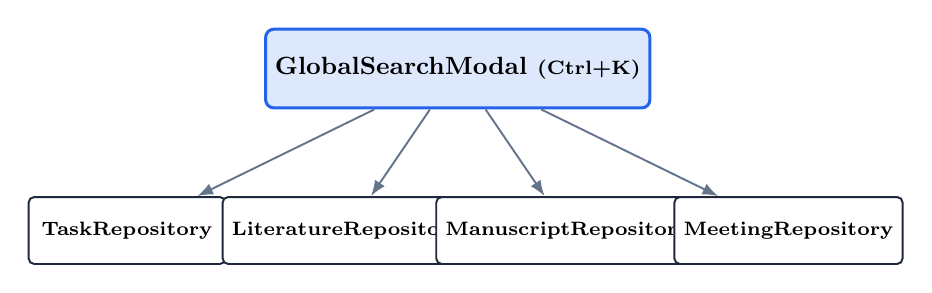
\begin{tikzpicture}[node distance=0.8cm]
    \node[hub, fill=crwblue!15] (modal) {GlobalSearchModal \scriptsize (Ctrl+K)};
    \node[ent, below=1.1cm of modal, xshift=-4.2cm] (t) {TaskRepository};
    \node[ent, below=1.1cm of modal, xshift=-1.4cm] (l) {LiteratureRepository};
    \node[ent, below=1.1cm of modal, xshift=1.4cm] (m) {ManuscriptRepository};
    \node[ent, below=1.1cm of modal, xshift=4.2cm] (mt) {MeetingRepository};
    \draw[arr] (modal) -- (t);
    \draw[arr] (modal) -- (l);
    \draw[arr] (modal) -- (m);
    \draw[arr] (modal) -- (mt);
  \end{tikzpicture}
  \vspace{0.4cm}
  \begin{itemize}\setlength\itemsep{5pt}
    \item A single query fans out across four repositories, scoped to the \textbf{active workspace} --- reuses the same \texttt{WorkspaceAccessGuard} check
    \item Demonstrates that the layered design \textbf{composes}: a feature spanning every module still respects one security boundary and one DTO contract
    \item Results are merged and ranked client-side before rendering in the modal
  \end{itemize}
\end{frame}

% ============================================================
\begin{frame}{Persistence Strategy}
  \begin{columns}[T,onlytextwidth]
    \column{0.5\textwidth}
      \textbf{File-backed H2}
      \begin{itemize}\setlength\itemsep{6pt}
        \item \texttt{jdbc:h2:file:./data/crwdb}
        \item Data survives backend restarts --- unlike a typical in-memory H2 demo setup
        \item Zero external DB dependency: clone, run, done
        \item \texttt{/h2-console} exposed (dev-only) for direct inspection
      \end{itemize}
    \column{0.5\textwidth}
      \textbf{Cascading \& ownership}
      \begin{itemize}\setlength\itemsep{6pt}
        \item \texttt{CascadeType.ALL} + \texttt{orphanRemoval=true} on Workspace$\to$Task, Manuscript$\to$Version, Literature$\to$Annotation
        \item Deleting a parent cleanly deletes its dependents --- no orphaned rows
        \item Lazy fetch by default everywhere; DTO mapping decides what actually gets pulled
      \end{itemize}
  \end{columns}
\end{frame}

% ============================================================
\begin{frame}{Architectural Principles, Distilled}
  \begin{columns}[T,onlytextwidth]
    \column{0.5\textwidth}
      \begin{itemize}\setlength\itemsep{8pt}
        \item[$\bullet$] \textbf{Separation of concerns} --- 5 uniform layers across 6 domains
        \item[$\bullet$] \textbf{Stateless security} --- JWT, no server session, scales horizontally
        \item[$\bullet$] \textbf{Defense in depth} --- role checks \emph{and} tenancy checks, independently
      \end{itemize}
    \column{0.5\textwidth}
      \begin{itemize}\setlength\itemsep{8pt}
        \item[$\bullet$] \textbf{Contract isolation} --- DTOs shield entities from the wire format
        \item[$\bullet$] \textbf{Uniform failure handling} --- one advice class, one error shape
        \item[$\bullet$] \textbf{Composable modules} --- global search proves the layers reuse cleanly
      \end{itemize}
  \end{columns}
  \vspace{0.6cm}
  \begin{center}
    \Large\textcolor{crwblue}{\textbf{A small feature set, built on patterns that scale to a much larger one.}}
  \end{center}
\end{frame}

% ============================================================
\begin{frame}{Thank You}
  \centering
  \vspace{0.6cm}
  {\Large \textbf{Questions?}}
  \vspace{0.8cm}

  \small
  \url{github.com/Rafat-Pantho/Centralized-Research-Workspace}

  \vspace{0.3cm}
  Team noWayHome --- Rafat Abdullah (220041102) \(\cdot\) Mahiul Kabir (220041109) \(\cdot\) Sohom Sattyam (220041141)
\end{frame}

\end{document}
